\documentclass[11pt,a4paper]{article}

% ---------- PAQUETES ----------
\usepackage[utf8]{inputenc}
\usepackage[T1]{fontenc}
\usepackage[spanish]{babel}
\usepackage[margin=2.5cm]{geometry}
\usepackage{graphicx}
\usepackage{url}
\usepackage[hidelinks]{hyperref}
\usepackage{booktabs}
\usepackage{listings}
\usepackage{xcolor}
\usepackage{caption}
\usepackage{float}

\lstset{
  basicstyle=\ttfamily\small,
  breaklines=true,
  frame=single,
  backgroundcolor=\color{gray!10}
}

\title{Herramientas CASE para Generación de Código: Visual Paradigm\\
\large Ingeniería de Requisitos (ISR-401)}
\author{}
\date{}

\begin{document}

% =========================================================
% 1. CARATULA
% =========================================================
\begin{titlepage}
\centering
{\large UNIVERSIDAD TÉCNICA ESTATAL DE QUEVEDO}\\
Facultad de Ciencias de la Computación y Diseño Digital\\
Carrera de Ingeniería en Software\\[1cm]
{\Large Ingeniería de Requisitos (ISR-401)}\\[0.3cm]
Docente: Ing. Gleiston Guerrero Ulloa, PhD.\\
Período académico: 2026--2027 PPA\\
Paralelo: [4to Software A]\\[1cm]
\rule{\linewidth}{0.4pt}\\[0.3cm]
{\LARGE\bfseries Herramientas CASE para Generación de Código:\\ Visual Paradigm}\\[0.3cm]
{\large Proyecto Fin de Curso: Sistema Inteligente de Mantenimiento de Palma Africana}\\[0.2cm]
\rule{\linewidth}{0.4pt}\\[1cm]
\begin{flushleft}
\centering\textbf{Integrantes:}\\
\centering Castro Bajaña Ariel Omar\\
\centering Mora Duarte Alex José\\
\centering Villafuerte Rosero Allan Noé\\
\centering Vera Gómez Anthony Alfredo
\end{flushleft}
\vfill
\sloppy
Repositorio: \url{https://github.com/AlanNVR/Grupo-C}
\end{titlepage}

% 2. RESUMEN (máx. 200 palabras)

\section*{Resumen}
[Pendiente: resumen ejecutivo del trabajo]

\newpage
\tableofcontents
\newpage

% 3. MARCO TEORICO  (Ariel Castro)

\section{Marco teórico}
\label{sec:marco-teorico}

\subsection{Model-Driven Engineering (MDE)}
\label{sec:mde}
El Model-Driven Engineering (MDE) es el paradigma de ingeniería de software en el que los modelos dejan de ser documentación de apoyo y pasan a ser artefactos de primera clase del proceso de desarrollo: la fuente autoritativa a partir de la cual se derivan, mediante transformaciones automatizadas, las implementaciones del sistema \cite{schmidt2006}. Bajo este enfoque, el esfuerzo de ingeniería se desplaza de la escritura manual de código hacia la definición precisa de modelos y de las reglas que los transforman, lo que favorece la trazabilidad, la reutilización y la reducción de errores de transcripción entre el diseño y la implementación. Trabajos recientes confirman que este desplazamiento no es solo teórico: Di Ruscio et al. \cite{diruscio2022} muestran que incluso las plataformas \textit{low-code} actuales —pensadas para usuarios sin formación técnica profunda— son, en esencia, una reencarnación práctica de los principios del MDE, lo que evidencia la vigencia y expansión industrial del paradigma.

\subsection{Model-Driven Architecture (MDA) y niveles de abstracción}
\label{sec:mda}

\subsection{Model-Driven Development (MDD)}
\label{sec:mdd}

\subsection{Transformaciones M2M y M2T}
\label{sec:m2m-m2t}

\subsection{Estado del arte y vigencia del enfoque}
\label{sec:estado-arte}

\section{Criterios éticos en el uso de herramientas de generación de código}
\label{sec:etica-ia}


\subsection{Transparencia: código generado vs. código escrito a mano}
\label{sec:transparencia}

\subsection{Licenciamiento del código generado}
\label{sec:licenciamiento}

\subsection{Sesgos y limitaciones de los generadores basados en IA generativa}
\label{sec:sesgos-ia}




% 4. JUSTIFICACION DE LA HERRAMIENTA (Allan Villafuerte)
\section{Justificación de la selección de la herramienta}

[Pendiente]

% 5. DESCRIPCION DEL SUBSISTEMA DEL PFC (Allan Villafuerte)

\section{Descripción del subsistema del PFC modelado}



% 6. MODELO UML DE ORIGEN (Allan Villafuerte)

\section{Modelo UML de origen}


\begin{figure}[H]
  \centering
  
  \caption{Diagrama de clases del subsistema [nombre].}
  \label{fig:diagrama-clases}
\end{figure}

Archivo nativo del modelo: \texttt{modelo/proyecto.vpp}.


% 7. CONFIGURACION DEL GENERADOR (Alex Mora)

\section{Configuración del mecanismo de generación}

% 8. PROCESO DE GENERACION (responsable: Alex Mora)

\section{Proceso de generación}

\begin{figure}[H]
  \centering

  \caption{Log de la generación de código en Visual Paradigm.}
\end{figure}

% 9. VERIFICACION DEL CODIGO GENERADO (responsable: Alex Mora)

\section{Verificación del código generado}

\begin{table}[H]
\centering
\caption{Correspondencia modelo $\rightarrow$ código generado.}
\begin{tabular}{llll}
\toprule
\textbf{Elemento UML} & \textbf{Tipo} & \textbf{Artefacto generado} & \textbf{Observación} \\
\midrule
% Clase X & Clase & X.java & OK \\
% Clase.atributoY & Atributo & campo + getter/setter & OK \\
\bottomrule
\end{tabular}
\end{table}

[Pendiente: limitaciones observadas del generador]

% =========================================================
% 10. CIERRE DEL CICLO / ROUNDTRIP (responsable: Anthony Vera)
% =========================================================
\section{Cierre del ciclo (roundtrip)}

\subsection{Cambio aplicado}
Para evidenciar el cierre del ciclo se seleccionó la clase Palma, entidad central del dominio del
sistema, y se le agregó el atributo fechaUltimoMantenimiento de tipo Date. Este cambio se
eligió por ser no trivial (posee tipo definido y no corresponde a un simple renombrado) y por su
pertinencia directa con el propósito del sistema: registrar la fecha de la última intervención de
mantenimiento realizada sobre cada palma monitoreada.
Tras aplicar el cambio en el modelo dentro de Visual Paradigm y validar su sintaxis, se
regeneró el código utilizando la misma plantilla y parámetros ya configurados en la Sección 7, sin
modificar la configuración del generador. El atributo nuevo se reflejó correctamente en la clase
generada, junto con sus métodos de acceso correspondientes (getFechaUltimoMantenimiento /
setFechaUltimoMantenimiento).

\begin{figure}[H]
    \centering
    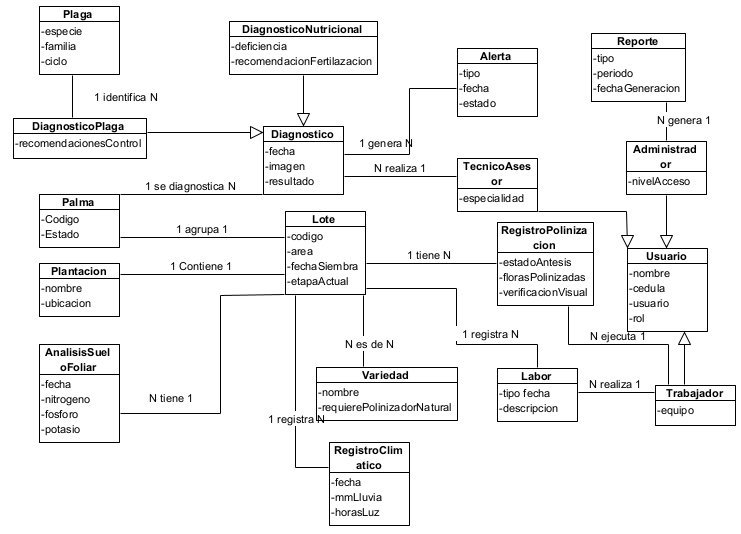
\includegraphics[width=0.45\textwidth]{figuras/modelo_antes.png}
    \hfill
    
\includegraphics[width=0.45\textwidth]{modelo_despues.png}
    \caption{Modelo antes (izquierda) y después (derecha) del cambio.}
    \label{fig:modelo_antes_despues}
\end{figure}

\begin{figure}[H]
  \centering
  
\includegraphics[width=0.45\textwidth]{codigo_antes.png}
    \hfill
    
\includegraphics[width=0.45\textwidth]{codigo_despues.png}
  \caption{Código generado antes (izquierda) y después (derecha) del cambio.}
\end{figure}

\begin{table}[H]
\centering
\caption{Trazabilidad del cambio aplicado (roundtrip).}

\resizebox{\textwidth}{!}{%
\begin{tabular}{llll}
\toprule
\textbf{Elemento UML} & \textbf{Tipo de cambio} & \textbf{Artefacto afectado} & \textbf{Resultado} \\
\midrule
Palma.fechaUltimoMantenimiento & Alta de atributo (DateTime) & Palma.java & OK, campo + getter/setter generados \\
\bottomrule
\end{tabular}%
}

\end{table}

% 11. REPARTO DEL TRABAJO (Anthony Vera)
\section{Reparto del trabajo por integrante}

\begin{table}[H]
\centering
\caption{Distribución de responsabilidades del equipo.}
\begin{tabular}{ll}
\toprule
\textbf{Integrante} & \textbf{Responsabilidad principal} \\
\midrule
Ariel Castro Bajaña & Marco teórico y criterios éticos de IA \\
Alex Mora Duarte & Configuración del generador, proceso de generación y verificación \\
Allan Villafuerte Rosero & Modelado UML, justificación de la herramienta \\
Anthony Vera Gómez & Roundtrip, documento LaTeX, organización del repositorio \\
\bottomrule
\end{tabular}
\end{table}

Enlace a commits por integrante: \url{https://github.com/AlanNVR/Grupo-C/commits/main/}


% 12. CONCLUSIONES
=
\section{Conclusiones}
% 
% 13. REFERENCIAS 

\section{Referencias}
\bibliographystyle{ieeetr}
\bibliography{referencias}

% =========================================================
% 14. ANEXOS 
\section*{Anexos}


\begin{figure}[H]
  \centering

  \caption{Captura de GitHub}
\end{figure}

\end{document}
